\documentclass[crop,tikz]{standalone}

\usepackage{libertinus}
\usepackage{libertinust1math}
\usepackage[T1]{fontenc}
\usepackage[scaled=0.79]{beramono}

\usetikzlibrary{positioning}
\usetikzlibrary{calc}
\usetikzlibrary{arrows.meta}

\begin{document}

\newlength\hdist\setlength\hdist{65mm}
\newlength\vdist\setlength\vdist{8mm}

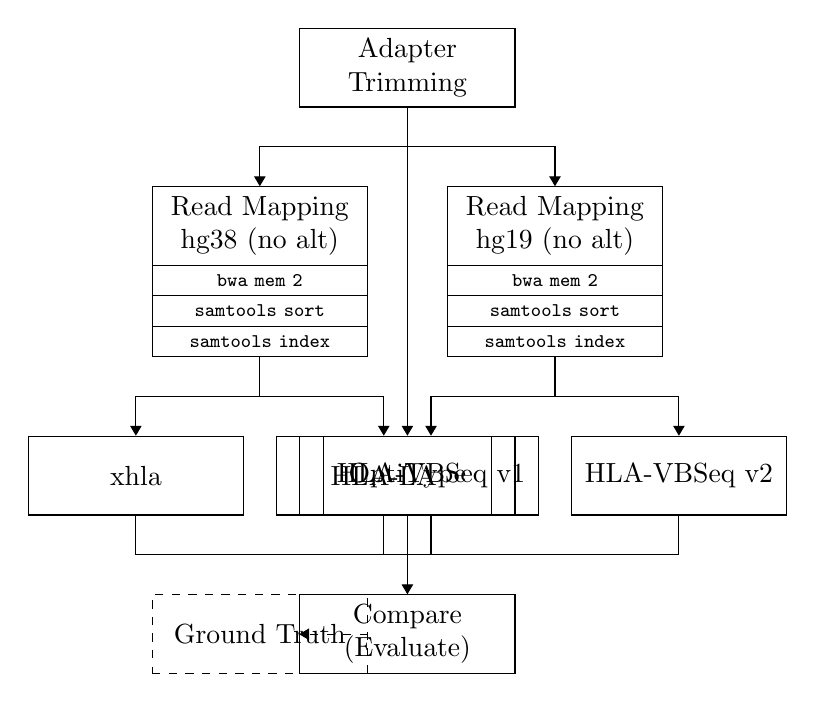
\begin{tikzpicture}[
    main/.style={
        draw,
        text width=25mm,
        align=center,
        minimum height=10mm,
    },
    minor/.style={
        main,
        minimum height=0mm,
        font=\ttfamily\scriptsize,
    }
    ]
    \node [main] (map38noalt) { Read Mapping\\hg38 (no alt)};
    \node [minor, below=-\pgflinewidth of map38noalt] (xhlaMap1) {bwa mem 2};
    \node [minor, below=-\pgflinewidth of xhlaMap1] (xhlaMap2) {samtools sort};
    \node [minor, below=-\pgflinewidth of xhlaMap2] (xhlaMap3) {samtools index};

    \node [main, below left=\vdist and 2mm of xhlaMap3, anchor=north] (xhla) {xhla};
    \node [main, below right=\vdist and 2mm of xhlaMap3, anchor=north] (hlala) {HLA-LA};
    \draw [-Triangle] (xhlaMap3.south) -- +(0,-.5\vdist) -| (xhla);
    \draw [-Triangle] (xhlaMap3.south) -- +(0,-.5\vdist) -| (hlala);

    \node [main,right=\hdist of map38noalt] (map19noalt) {Read Mapping\\hg19 (no alt)};
    \node [minor, below=-\pgflinewidth of map19noalt] (vbseqMap1) {bwa mem 2};
    \node [minor, below=-\pgflinewidth of vbseqMap1] (vbseqMap2) {samtools sort};
    \node [minor, below=-\pgflinewidth of vbseqMap2] (vbseqMap3) {samtools index};

    \node [main, below left=\vdist and 2mm of vbseqMap3, anchor=north] (vbseq1) {HLA-VBSeq v1};
    \node [main, below right=\vdist and 2mm of vbseqMap3, anchor=north] (vbseq2) {HLA-VBSeq v2};

    \draw [-Triangle] (vbseqMap3.south) -- +(0,-.5\vdist) -| (vbseq1);
    \draw [-Triangle] (vbseqMap3.south) -- +(0,-.5\vdist) -| (vbseq2);

    \node [main] (optitype) at ($(hlala)!.5!(vbseq1)$) {OptiType};

    \node [main, anchor=south] (trim) at ($(map38noalt.north west)!.5!(map19noalt.north east) + (0,\vdist)$) {Adapter Trimming};
    \draw [-Triangle] (trim) -- (optitype);

    \draw [-Triangle] (trim.south) -- +(0,-.5\vdist) -| (map19noalt.north);
    \draw [-Triangle] (trim.south) -- +(0,-.5\vdist) -| (map38noalt.north);

    \node [main, below=\vdist of optitype] (compare) {Compare (Evaluate)};

    \draw [-Triangle] (xhla.south) |- ($(compare.north)+(0,.5\vdist)$) -- (compare.north);
    \draw (hlala.south) -- +(0,-.5\vdist);
    \draw (optitype.south) -- +(0,-.5\vdist);
    \draw (vbseq1.south) -- +(0,-.5\vdist);
    \draw (vbseq2.south) |- ($(compare.north)+(0,.5\vdist)$) -- (compare.north);

    \coordinate (ref) at ($(xhla.south)!.5!(hlala.south)$);
    \node [main, dashed, below=\vdist of ref] (gstandard) {Ground Truth};
    \draw [dashed, -Triangle] (gstandard) -- (compare);
\end{tikzpicture}

\end{document}
